
\section{mtra2g.rb - Construct item similarity graph\label{sect:mtra2g}}

This command constructs a general graph (referred to as "similarity graph") to reflect the structural similarity between items within the transaction data . 
The \verb|lcm|  \cite{UnoWeb}  command is used in mtra2g.rb.  
Degree of similarity is defined by the co-occurrence information of two items, by extending an edge between items a similarity measure higher than the lower limit specified by the user.
Probability of item occurrence (support) and number of occurrence can be specified to derive degree of similarity. In addition, resemblance and the normalized PMI can be added as additional criteria. The definition of each is shown in Table \ref{tbl mt2g_simdef}.


\begin{table}[htbp]
\begin{center}
\caption{Definition of degree of similarity between items $a$ and $b$ \label{tbl:mt2g_simdef}}
%{\small
\begin{tabular}{cllcc}
\hline
Degree of similarity&Formula&Parameter&Range \\
\hline
support        & $\frac{|Occ(a,b)|}{n}$ & s= & 0.0〜1.0 \\
occurence      & $|Occ(a,b)|$ & S= & 1〜 \\
recemblance    & $\frac{|Occ(a) \cap Occ(b)|}{|Occ(a) \cup Occ(b)|}$ & sim=R th= & 0.0〜1.0\\
normalized PMI & $\log{\frac{P(a,b)}{P(a)P(b)}}/(-\log{P(a,b)})$ & sim=P th=  & -1.0〜1.0\\
               & $=\frac{n|Occ(a) \cap Occ(b)|}{|Occ(a)||Occ(b)|}/(-\log{\frac{|Occ(a) \cap Occ(b)|}{n}})$ & \\
\hline
\end{tabular} 
\\
{\scriptsize
$n$ represents the total number of transactions. 
$Occ(a)$ represents the transaction set which item a appeared. 
$P(a)$ represents the probability of occurrence for item a denoted as $P(a)=Occ(a)/n$.
}
\end{center}
\end{table}

The same key-based transaction data is used as the input data used in \hyperref[sect:mitemset]{mitemset.rb} command is used as input data in this section as shown in (Table \ref{tbl:mt2g_key}). 
The data is converted from key based to transaction based formatted data by \verb|mtra| command in MCMD package as shown in Table \ref{tbl:mt2g_tra}. 

Given the input data, Table \ref{tbl:mt2g_out1} shows the result of similarity graph with 2 or more  occurrence, the graph structure is shown in Figure \ref{fig:mt2g_out1} . 


\begin{table}[htbp]
\begin{center}
\begin{tabular}{ccc}

\begin{minipage}{0.25\hsize}
\begin{center}
\caption{Key based data\label{tbl:mt2g_key}}
{\small
\begin{tabular}{cc}
\hline
key&item \\
\hline
T1&C \\
T1&E \\
T2&D \\
T2&E \\
T2&F \\
:&: \\ \hline
\end{tabular} 
}
\end{center}
\end{minipage}

\begin{minipage}{0.25\hsize}
\begin{center}
\caption{Tra based data\label{tbl:mt2g_tra}}
{\small
\begin{tabular}{ll}
\hline
id&item \\
\hline
T1&C E \\
T2&D E F \\
T3&A B D F \\
T4&B D F \\
T5&A B D E \\
T6&A B D E F \\
\hline
\end{tabular} 
}
\end{center}
\end{minipage}

\begin{minipage}{0.5\hsize}
\begin{center}
\caption{Item similarity graph with 2 or more occurrence. The probability of occurrence indicates the number of occurrence. When sim= parameter is specified, the value will be shown in the final column (void). 
\label{tbl:mt2g_out1}}
{\small
\begin{tabular}{cccc}
\hline
node1&node2&support&void\\
\hline
a&b&0.6&\\
a&d&0.4&\\
a&f&0.4&\\
d&b&0.6&\\
e&d&0.4&\\
f&b&0.6&\\
f&d&0.6&\\
\hline
\end{tabular} 
}
\end{center}
\end{minipage}


\end{tabular} 
\end{center}
\end{table} 

\begin{figure}[htbp]
\begin{center}
\begin{minipage}{0.3\hsize}
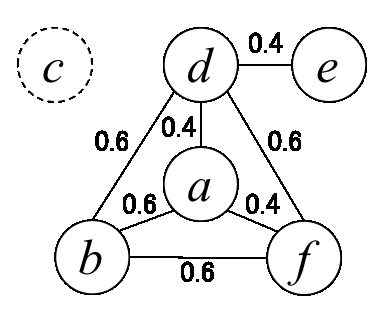
\includegraphics[scale=0.6]{./simg.eps}
\caption{The corresponding similarity graph is shown in Figure \ref{tbl:mt2g_out1}. Each edge shows the co-occurrence probability of the two items. \label{fig:mt2g_out1}}
\end{minipage}
\end{center}
\end{figure}


\subsection{Format}
\begin{verbatim}
Format) mtra2g.rb i= tid= item= [on=] oe= s= [sim=] [th=] [log=] [T=] [--help]

  Specification of file name
  i=     : Transaction data file 
  tid=   : Field name of Transaction ID
  item=  : Field name of item 
  on=    : Output file (node)
  oe=    : Output file (side:node pair)
  s=     : Minimum support [(specified by percentage of total number of transactions): real number between 0 and 1]
  S=     : Minimum support [(specify the number of transactions): integer above 1]
         : When both s=,S= is not specified, default setting becomes S=1. 
  sim=   : Degree of similarity
           R: resemblance
           P: normalized PMI
           When not specified, the edge is extended based on the criteria specified at s= and S=. 
  th=    :  Extend an edge between items with the degree of similarity above  the threshold value specified here. Type of degree of similarity is specified at sim=.
 log=   : Specify file name to save the parameter settings in key-based CSV format. 

  Others
  T= : Working directory (default:/tmp)
  --help : Help information 
\end{verbatim}

\subsection{Examples}
\subsubsection*{例1: 基本例}

出現件数が2件以上の類似度グラフ。
上述の解説の中で示した例。


\begin{Verbatim}[baselinestretch=0.7,frame=single]
$ more dat1.csv
tid,item
T1,C
T1,E
T2,D
T2,E
T2,F
T3,A
T3,B
T3,D
T3,F
T4,B
T4,D
T4,F
T5,A
T5,B
T5,D
T5,E
T6,A
T6,B
T6,D
T6,E
T6,F
$ mtra2g.rb  S=2 tid=tid item=item i=dat1.csv eo=edge1.csv
#MSG# converting a named item into a numbered item ...
#MSG# run lcm enumerating 2 itemset ...
#MSG# creating the edge file ...
#END# /usr/bin/mtra2g.rb S=2 tid=tid item=item i=dat1.csv eo=edge1.csv
$ more edge1.csv
node1,node2,support,void
A,B,0.5,
A,D,0.5,
A,E,0.3333333333,
A,F,0.3333333333,
B,D,0.6666666667,
E,B,0.3333333333,
E,D,0.5,
F,B,0.5,
F,D,0.6666666667,
F,E,0.3333333333,
\end{Verbatim}
\subsubsection*{例2: resemblanceを追加}

例1に加えてresemblanceが0.4以上を類似度条件に加える。
また\verb|no=|を指定することで、節点情報としてアイテム単独の出現頻度を出力する。


\begin{Verbatim}[baselinestretch=0.7,frame=single]
$ mtra2g.rb  S=2 sim=R th=0.4 tid=tid item=item i=dat1.csv eo=edge2.csv no=node2.csv
#MSG# converting a named item into a numbered item ...
#MSG# run lcm enumerating 2 itemset ...
#MSG# creating the edge file ...
#MSG# creating the node file ...
#END# /usr/bin/mtra2g.rb S=2 sim=R th=0.4 tid=tid item=item i=dat1.csv eo=edge2.csv no=nod
e2.csv
$ more node2.csv
node,support
A,0.5
B,0.6666666667
C,0.1666666667
D,0.8333333333
E,0.6666666667
F,0.6666666667
$ more edge2.csv
node1,node2,support,resemblance
A,B,0.5,0.75
A,D,0.5,0.6
A,E,0.3333333333,0.4
A,F,0.3333333333,0.4
B,D,0.6666666667,0.8
E,D,0.5,0.5
F,B,0.5,0.6
F,D,0.6666666667,0.8
\end{Verbatim}



